% !TEX program = xelatex

\documentclass{resume}
%\usepackage{zh_CN-Adobefonts_external} % Simplified Chinese Support using external fonts (./fonts/zh_CN-Adobe/)
%\usepackage{zh_CN-Adobefonts_internal} % Simplified Chinese Support using system fonts
\usepackage{tabu}

\begin{document}
\pagenumbering{gobble} % suppress displaying page number

\begin{minipage}{0.7\textwidth}
  \Large{
    \begin{tabu}  { l }
      \scshape{Jingtao Zhang} \\
      \email{sy1906605@buaa.edu.cn} \\
      \phone{(+86) 178-5416-0892} \\
    \end{tabu}
  }
\end{minipage}
\begin{minipage}{0.3\textwidth}
  \raggedleft
  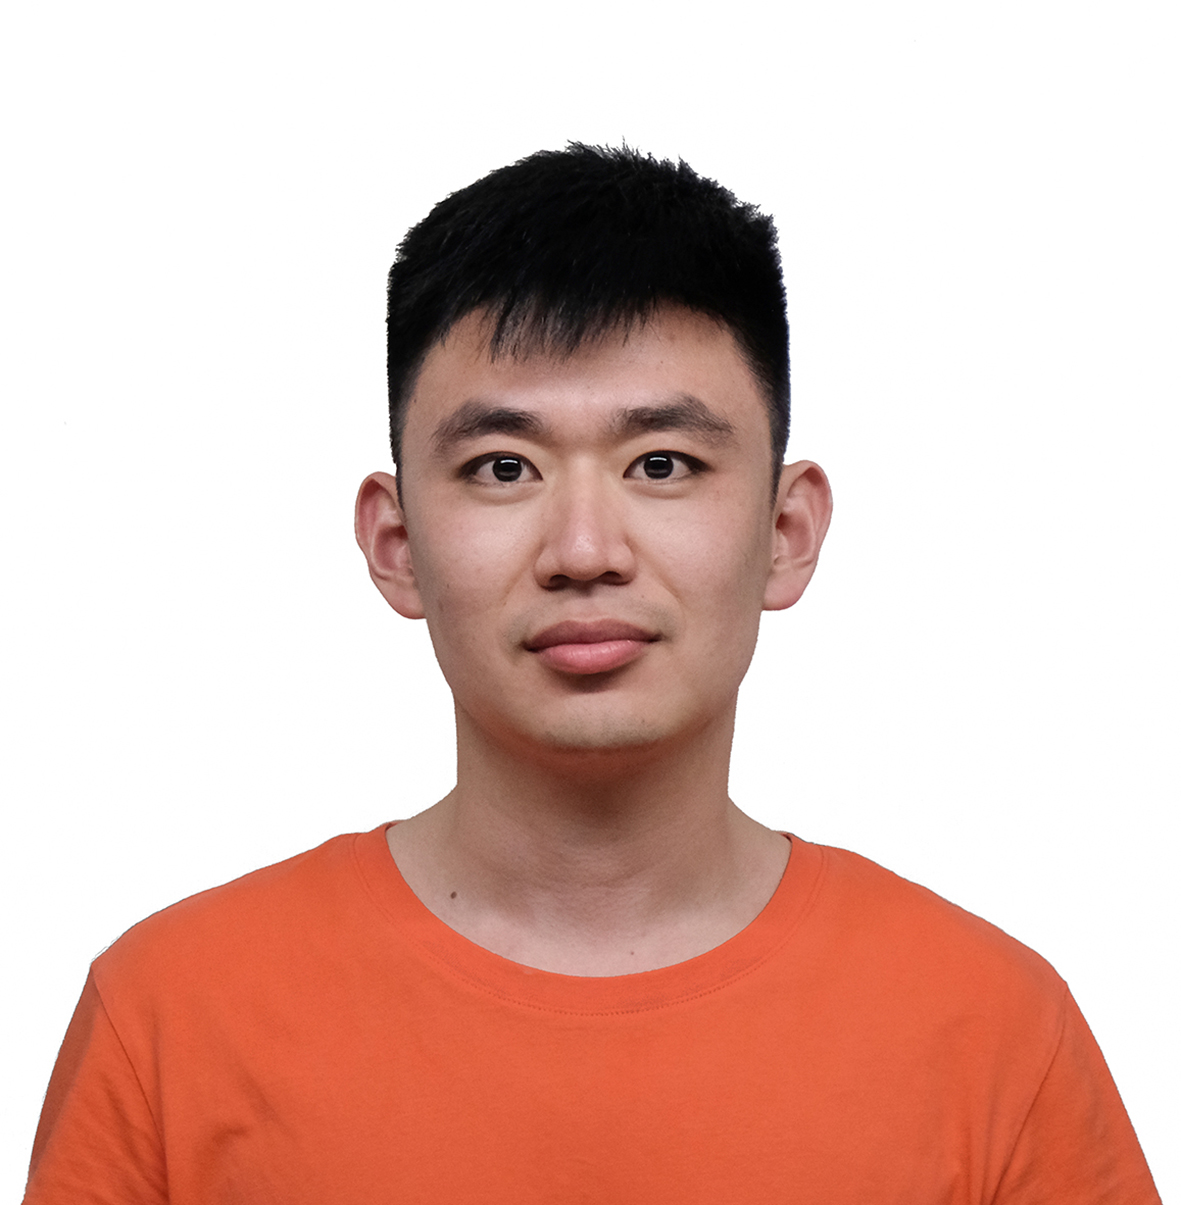
\includegraphics[height=30mm]{avatar}
\end{minipage}

\section{\faGraduationCap\ Education}
\datedsubsection{\textbf{Beihang University (BUAA)}, Beijing, China}{2019 -- Present}
Master of Computer Science and Technology(CS),\ expected Jan. 2022
\datedsubsection{\textbf{Shandong University (SDU)}, Jinan \& Qingdao, China}{2015 -- 2019}
Bachelor of Computer Science and Technology(CS),\ (GPA4.68/5.0, top2\%)

\section{\faUsers\ Experience}

\datedsubsection{\textbf{Beijing Renaissance Era Investment Co., Ltd}}{Apr. 2020 - Sept. 2020}
\role{Back-end Developer Intern}{}
Participate in the construction and maintenance of Serverless Function, transform fission function framework based on knowing Kubernetes cluster, and extend the transformation to the company:
\begin{itemize}[topsep = 0 pt, partopsep = 0pt]
  \item Simplify the process for developers to write and deploy functions and provide function creation template, local test environment and automatic deployment script to make developers who are not familiar with Kubernetes can write and deploy their services after simple training.
  \item Enrich the functions of Fission, including improving log viewer and delivery, adding level configuration of functions and data flow visualization component, etc., which facilitates user debugging, simplifies the process of function migration from the test environment to the production environment, and shows the data flow of the whole project clearly.
  \item Details can be found in the project of \href{https://github.com/jingtaozhang18/fission}{Fission} and \href{https://github.com/jingtaozhang18/fission-template}{Fission Template} and its \href{https://jingtao.fun/%E6%BA%90%E7%A0%81-Fission%E5%8A%9F%E8%83%BD%E6%8B%93%E5%B1%95/}{file} of transformation summary (publicly approved by BREI Co., Ltd).
\end{itemize}

\datedsubsection{\textbf{Beijing Zitiao Network Technology Co., Ltd}}{Mar. 2019 - Sept. 2019}
\role{Toutiao Back-end Developer Intern}{}
\begin{itemize}[topsep = 0 pt, partopsep = 0pt]
  \item Participate in the maintenance of monitoring alarm platform, including real-time processing of log stream (> 1mil / s) and regular query of data index. Process the log flows by the computing engine and write them into ES, Metrics and Druid storage engines, and obtain the indicators of monitoring data by the regular query.
  \item Participate in the construction of automatic internal test system, including the maintenance of internal test user pool, the portrait construction of internal test user, reward mechanism and the evaluation of internal test effect. Develop the function of automatically supplementing internal test user pool, calculate internal test effect, display module, etc.
\end{itemize}

% \datedsubsection{\textbf{Developer of a small movie recommender}}{2018.03 - 2018.06}
% \role{Shandong University }{Independent Design}
% \begin{itemize}[topsep = 0 pt, partopsep = 0pt]
%   \item Develop a small movie recommender based on collaborative filtering, which can deal with different scoring preferences of different users.
%   \item The system is based on spark big data framework and implemented with Scala programming language.
% \end{itemize}

% \datedsubsection{\textbf{Develop the Intelligence SDU, a convenient campus service system with group members. }}{2016.06 - 2017.10}
% \role{Shandong University\ Qilu software competition}{Team Leader}
% \begin{itemize}[topsep = 0 pt, partopsep = 0pt]
%   \item The project is based on the PHP framework of Laravel, using the form of web pages, providing students with the service of query, repair, forum, automatic course selection, personal network disk, reminding of new notice from important websites, etc.
%   \item Develop the API docking with the official website of Shandong University (including student identity authentication, automatic crawler comparison of important websites, etc.); create and maintain database system and assemble the cloud disk and forum modules; build the whole system on the cloud server and test it.
% \end{itemize}

\section{\faCogs\ Skills}
\begin{itemize}[parsep=0.5ex]
  \item Programming Languages: C++ Python Go
  \item Tools: Linux Git Docker
  \item Languages: English-CET6
\end{itemize}

\section{\faHeartO\ Honors and Awards}
\datedline{\textit{National scholarship}}{2017 \& 2018}
\datedline{\textit{Excellent Student Leaders of SDU}}{2016 \& 2017}
\datedline{\textit{\nth{3} International Hardware Design Contest}}{2017}
\datedline{\textit{\nth{1} Software Design Competition for college students in Shandong Province}}{2017}
\datedline{\textit{\nth{2} Mathematical Contest in Modeling in Shandong area}}{2017}

% \section{\faInfo\ Miscellaneous}
% \begin{itemize}[parsep=0.5ex]
%   \item Blog: http://jingtao.fun
%   \item GitHub: https://github.com/jingtaozhang18
% \end{itemize}

\end{document}
